\RequirePackage{etex} %% **************** add this for ARXIV submission
\documentclass[runningheads,twocolumn,a4paper,10pt]{llncs}
% \documentclass[runningheads,a4paper]{llncs}
% \usepackage{threeparttable}
% \usepackage{hyperref}
% \usepackage[colorlinks,citecolor=blue]{hyperref}
% \usepackage{draftwatermark}
% \usepackage[maxnames=3,firstinits=true,sorting=none,doi=false,url=true,isbn=false]{biblatex}
% \usepackage[maxnames=6,firstinits=true,doi=false,url=true,isbn=false]{biblatex}
% \addbibresource{../source/refs.bib}

\usepackage{etex}
\reserveinserts{28}
\pdfoutput=1
\setcounter{tocdepth}{3}
\usepackage[a4paper, total={7in, 10in}]{geometry}
% \usepackage[linesnumbered,lined,boxed,commentsnumbered,ruled]{algorithm2e}
% \renewcommand{\algorithmcfname}{ALGORITHM}
% \SetAlFnt{\small}
% \SetAlCapFnt{\small}
% \SetAlCapNameFnt{\small}
% \SetAlCapHSkip{0pt}
% \IncMargin{-\parindent}
\usepackage{ textcomp }
\usepackage{ comment }
\usepackage[color=yellow!60,textsize=footnotesize,obeyDraft,draft]{todonotes}
\usepackage{colortbl}
\usepackage{booktabs}
% \usepackage[pdftex]{graphicx}
\usepackage{tabularx}
\usepackage{capt-of}
\usepackage{makecell}
\usepackage{multirow}
\usepackage{listings}
% \usepackage{graphicx}
\usepackage{amsmath}
\usepackage{caption}
\usepackage{subcaption}
\usepackage[font=footnotesize,labelfont=bf]{subcaption}
\usepackage[hidelinks]{hyperref}
\usepackage[capitalize]{cleveref}
\captionsetup{compatibility=false}
\usepackage{tikz}
\usepackage{pgfplots}
\pgfplotsset{compat=newest}
\pgfplotsset{plot coordinates/math parser=false}
\usepackage[para,online,flushleft]{threeparttable}
\usepackage{wasysym}
\usepackage{amssymb}
\usetikzlibrary{arrows}
% \usepackage{subfig}
\usepackage{breakcites}
\usepackage{array}
\usepackage{color}
\usepackage{balance} %balance columns
\usepackage{lastpage}
\hyphenation{op-tical net-works semi-conduc-tor}
\usepackage{dblfloatfix}
\usepackage{authblk}
% \usepackage[disable]{todonotes}
\usepackage{siunitx}
\usepackage{xurl} %for long URLs
\usepackage[shortlabels]{enumitem}
\usepackage{soul}
% \usepackage[dvipsnames]{xcolor}
\usepackage{xcolor,listings}
\usepackage{relsize}
\usepackage{algorithm}
\usepackage{algpseudocode}

% for caption at top of table
\usepackage{float}
\floatstyle{plaintop}
\restylefloat{table}
\setcounter{secnumdepth}{3}
\lstset{upquote=true}

% Packages for drawing
\usepackage{tikz}
\usetikzlibrary{shapes.geometric, arrows,calc}
\tikzstyle{startstop} = [rectangle, rounded corners, minimum width=3cm, minimum height=1cm,text centered, draw=black, fill=none]
\tikzstyle{io} = [trapezium, trapezium left angle=70, trapezium right angle=110, minimum width=3cm, minimum height=1cm, text centered, draw=black, fill=blue!30]
\tikzstyle{process} = [rectangle, minimum width=3.5cm, minimum height=1cm, text centered, draw=black, fill=orange!0]
\tikzstyle{neuron} = [circle, minimum size=3cm, text centered, draw=black, fill=orange!0]
\tikzstyle{decision} = [diamond, minimum width=3cm, minimum height=1cm, text centered, draw=black, fill=green!30]
\tikzstyle{arrow} = [thick,->,>=stealth]


\usepackage[maxnames=6,firstinits=true,doi=false,url=true,isbn=false]{biblatex}
\addbibresource{netzip_arxiv.bib}

\def \assumptionSGDfirst {1}
\def \assumptionEWCfirst {2}
\def \assumptionEWCsecond {3}

\pagenumbering{arabic}


\begin{document} 

% \title{Towards a Measure of Trustworthiness to Evaluate CNNs During Operation}
\title{Evaluation Metrics for CNNs Compression}%A Measure of Trustworthiness to Evaluate CNNs Predictions}
\titlerunning{Evaluation Metrics for CNNs Compression}
\authorrunning{Ghobrial et al.}

\author{Abanoub Ghobrial\inst{1}, Dieter Balemans\inst{2}, Hamid Asgari\inst{3}, Phil Reiter\inst{2}, Kerstin Eder\inst{1}}

\institute{University of Bristol, Bristol, UK \and University of Antwerp, Antwerp, Belgium \and Thales, Reading, UK}
\tocauthor{Authors' Instructions}

\maketitle
% \let\thefootnote\relax\footnotetext{
% Abanoub Ghobrial (e-mail: abanoub.ghobrial@bristol.ac.uk), 
% and 
% Kerstin Eder (e-mail: kerstin.eder@bristol.ac.uk) 
% are with the Trustworthy Systems Lab, Department of Computer Science, University of Bristol, Merchant Ventures Building, Woodland Road, Bristol, BS8 1UB, United Kingdom.
% %
% Dieter Balemans (e-mail:) and Phil Reiter (e-mail:) 
% %
% Hamid Asgari (e-mail: hamid.asgari@uk.thalesgroup.com) 
% is with Technology and Innovation Research,Thales, Reading, United Kingdom.}

%
\makeatletter
\renewcommand\subsubsection{\@startsection{subsubsection}{3}{\z@}%
                       {-18\p@ \@plus -4\p@ \@minus -4\p@}%
                       {4\p@ \@plus 2\p@ \@minus 2\p@}%
                       {\normalfont\normalsize\bfseries\boldmath
                        \rightskip=\z@ \@plus 8em\pretolerance=10000 }}
\makeatother

\textbf{\textit{Abstract}--There is a lot of research effort into developing different techniques for neural networks compression. However, the community lacks standardised evaluation metrics, which are key to identifying the most suitable compression technique for different applications. 
%
This paper reviews existing neural network compression evaluation metrics and implements them into a standardisation framework called NetZIP.% Which provides a robust neural network compression benchmark.
%
We introduce two novel metrics to cover existing gaps of evaluation in the literature: 1) Compression and Hardware Agnostic Theoretical Speed (CHATS) and 2) Overall Compression Success (OCS).
%
We demonstrate the use of NetZIP using two case studies on two different hardware platforms (a PC and a Raspberry pi 4) focusing on object classification and object detection.}

% ***************************************************
%  Main Body
% ***************************************************
\section{Introduction}

% == The Challenge -> to raise importance for CNNs compression.
State-of-the-art Deep Neural Networks (DNNs) are becoming the go-to solution in computer vision for automated systems operating in complex high dimensional domains. 
%
Achieving high accuracy of DNN models during training usually come at the expense of overparameterizing the model~\cite{Neill2020}.
%
This results in well performing DNNs that are oversized. 
%
Being oversized hinders the deployment of DNN models on low-size weight and power (SWaP) edge devices, as well as having an unnecessary large carbon footprint during operation.
%
These issues are expected to get worse as the complexity of operational environments increase and thus the models will consequently need to be larger, making the deployment even more challenging~\cite{Marino2023, Brown2020}.  

% == Introduce Deep Neural Network Compression
A possible solution is to take an adaptive approach, where a smaller model is trained on a subset of the operational environment and then adapted depending on shifts in the environment e.g.~\cite{Ghobrial2022, mirza2022norm}.
%
These approaches present their own questions regarding information forgetting, resource requirements and energy consumption.
%
Also, whilst this may assist with the problem of needing to increase the model size as the operational environment increases,
% increasing operational envionrnments deploying models on to low resource computers.
the neural network will still be oversized compared to the amount of information retained at one time. 

Therefore, \textit{neural network compression} has recently seen a surge in its research outputs, as compression offers significant reduction in size and energy consumption whilst aiming to retain the same overall accuracy performance and improving the speed of predictions. 
%
% == Brief overview on existing CNN compression techniques. Highlight on Quantisation and Pruning if adequate.
There are many compression techniques in the literature that fall under one of these compression categories: pruning, quantisation, knowledge distillation and tensor decomposition. These different categories are nicely discussed in these two reviews \cite{Neill2020}\cite{Marino2023}.
%
% == Elaborate on the need for standardisation between these techniques.
Most research efforts has focused on developing compression techniques but the community seems to lack a standardised way of evaluation between different compression techniques.

  
% Goal of NEtzip is standardising evaluation of DNN Quantisation. Netzip also facilitates the usage of ShrinkBench is a standardisation library for pruning methods, which allows users to compare between pruning and quantisation techniques.  

% Unlike TensorFlow which may support integer quantization using arbitrary bit-width from 2 to 16, PyTorch only supports bit-widths of 8 according the this blog: \url{https://leimao.github.io/blog/PyTorch-Quantization-Aware-Training/}


% In our case study we focus on CNNs, however, in our future works we plan to extend this to include LSTMs transformers  etc. (use this link from pytorch to help categorise the different types of DNNs: https://pytorch.org/docs/stable/quantization.html\#general-quantization-flow)
% \subsection{Motivation}

% Why is it important to standardise?
Based on a recent review, most of the methods in the literature do not compare their compression techniques with existing techniques and where comparisons are made they tend to vary between different publications~\cite{Blalock2020}.
%
This is largely due to the lack of standardised implementation of metrics, neural networks, and compression techniques. 
%
In this paper, we focus predominantly on the metrics aspect.
%
The contributions of this paper are three folds: 
% \begin{enumerate}
    % \item 
    1) Provide a review of evaluation metrics used to assess compression techniques. 
    % \item 
    2) Identify gaps in evaluation metrics and contribute metrics to fill these gaps.
    % \item 
    3) Using the reviewed and our developed evaluation metrics, we introduce NetZIP, a growing standardized benchmark library for comparing compression techniques available at \url{https://github.com/TSL-UOB/NetZIP}. NetZIP is aimed to help users identify the most suitable compression technique for their trained neural network using several baseline compression techniques, and also serve to compare newly developed compression techniques against others.%some standard compression techniques and CNNs. 
% \end{enumerate}
%

The paper is organised as follows, in section~\ref{sec:background} we overview compression methods and existing compression benches. We provide our review of evaluation metrics and our novel metrics in section~\ref{sec:metrics}. Section~\ref{sec:NetZIP_overview} introduces NetZIP and section~\ref{sec:casestudies} showcases comparisons made using NetZIP. Conclusions and futures work are provided in section~\ref{sec:Conclusions}.

\begin{figure*}
    \centering
    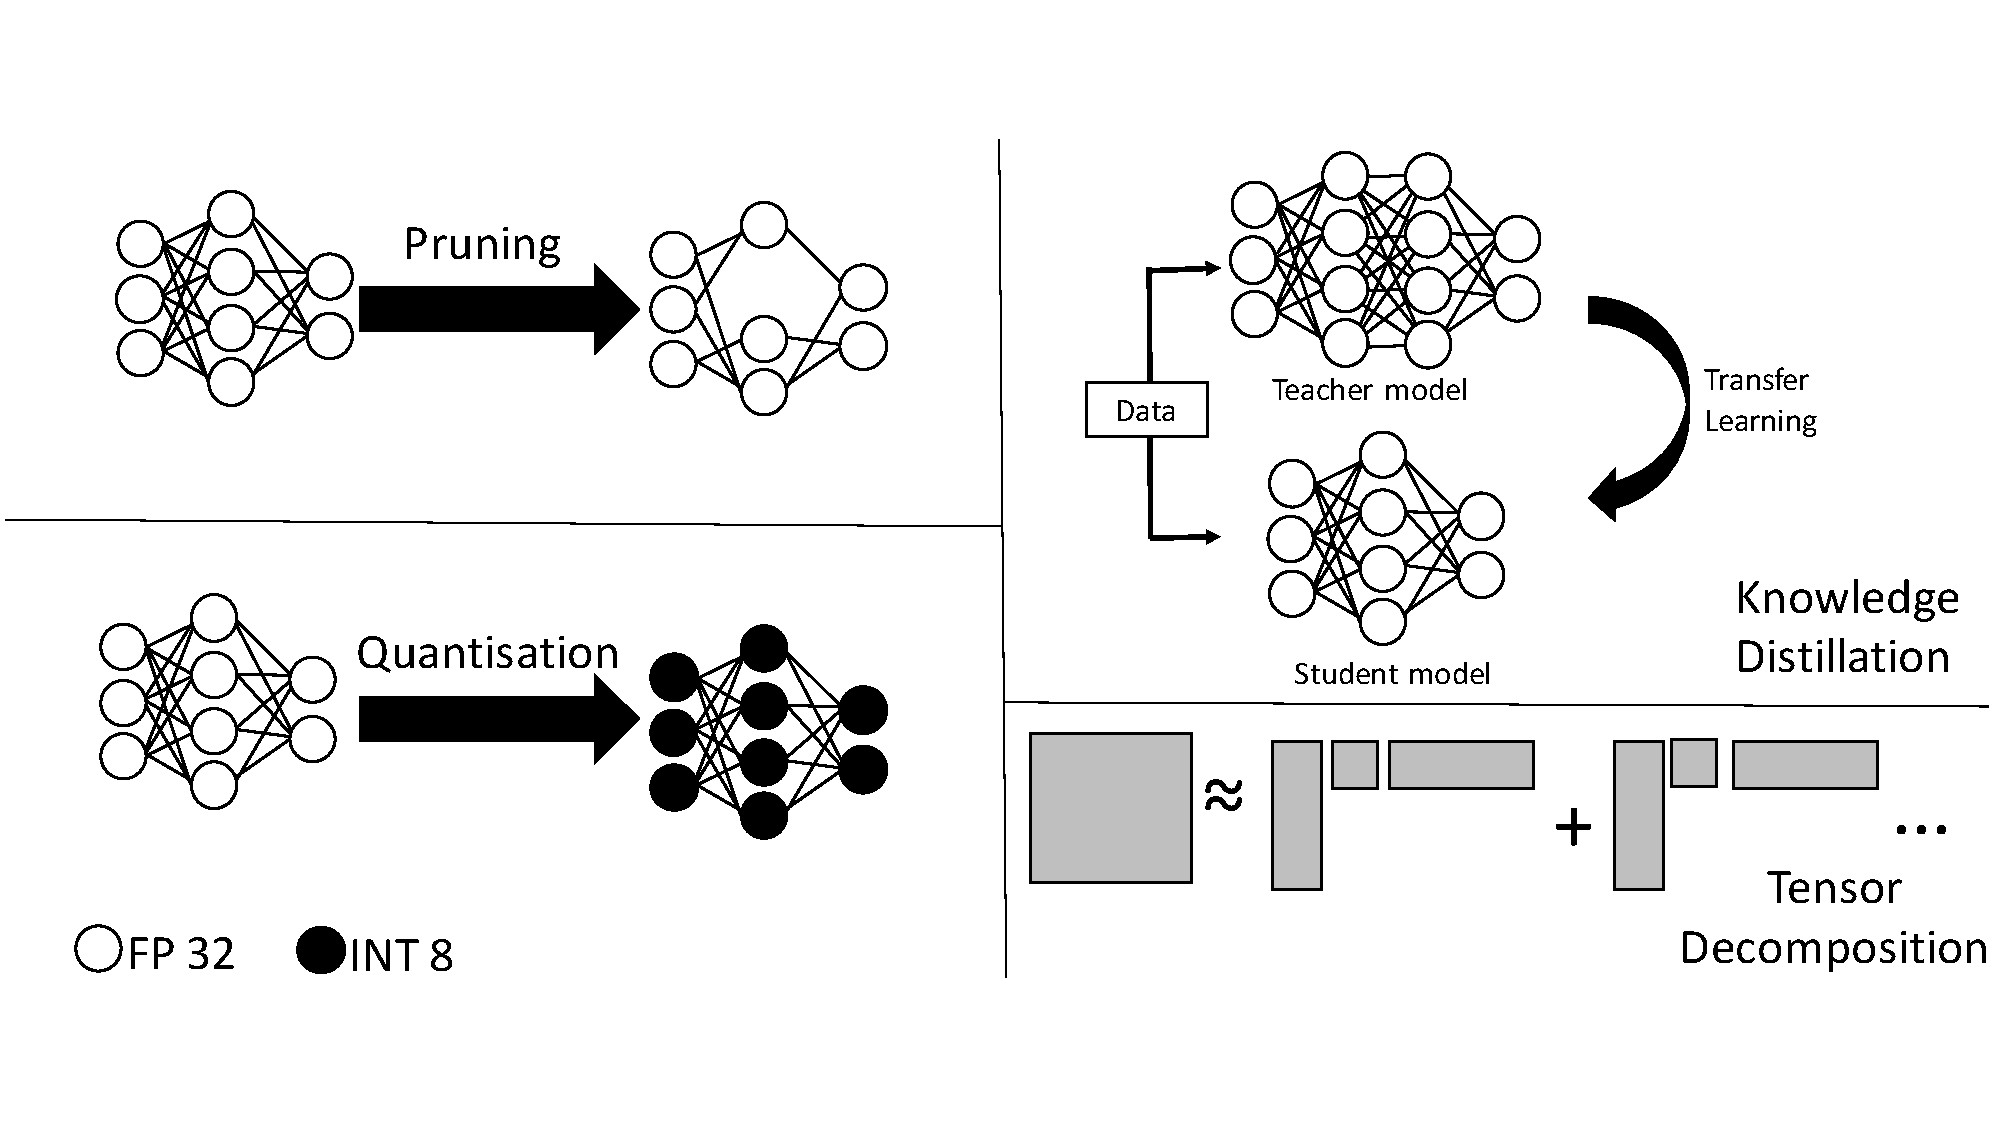
\includegraphics[width=1\textwidth]{other/figures/compression_methodsv2.pdf}{}
    \caption{Shows an overview of the four compression techniques categories currently available in the literature. The four categories are Pruning, Quantisation, Knowledge Distillation and Tensor Decomposition.}
    \label{fig:compression_methods}
\end{figure*}

% Why compression? 

% -Decreases model size.

% -Decreases energy consumption.

% -Increases Speed.

% Reduced computational requirements: Smaller models require fewer resources to train and deploy, which can significantly reduce the computational requirements and energy consumption.

% Improved memory and storage efficiency: Smaller models require less memory and storage space, which can be particularly useful in scenarios where resources are limited, such as mobile devices or edge computing.

% Faster inference: Smaller models can perform inference faster, which is particularly important in real-time applications such as object detection and autonomous driving.


% Why standardised compression bench.
% Effectiveness of compression can vary due to~\cite{Blalock2020}:
% Blalock et.al.~\cite{Blalock2018} 

% -Variations in initializations. 

% -Initial model training.

% -Different Implementation of deep learning libraries.
% \subsection{Contribution and Organisation of paper}




% =====

% Whilst NetZIP is meant to be a growing toolkit library, currently we currently focus on deep neural networks for vision tasks, with the scope of expanding to natural language processing applications and other fields needed by the community. 

% NetZIP is an open-source bench marking framework for evaluating the performance of model compression techniques on deep neural networks. It provides a standardized set of benchmarks and evaluation metrics for comparing different compression methods.
%
% NetZIP allows for training models from scratch or using pre-trained models  to evaluate compression techniques. It also includes a suite of compression methods, mainly pruning and quantization, which can be easily applied to the pre-trained models.
%
% The framework provides a range of evaluation metrics to measure accuracy, speed, size, and energy which can be used to assess the performance of the compressed models. 
%
% NetZIP is designed to be easily extensible, allowing researchers and developers to add their own models and compression techniques to the benchmarking suite. 
% Overall, NetZIP provides a standardized framework for evaluating the performance of model compression techniques, enabling researchers and developers to more easily compare and evaluate different methods.



% \begin{enumerate}
    % \item Identify the most suitable compression technique for their trained Neural Network using several (baseline) compression techniques.
    % \item Compare newly developed compression techniques against some standard compression techniques and CNNs.
% \end{enumerate}

% Mention that this compression bench is in continuous development and will continue to evolve over time. 

% \section{Definitions (~0.5 pages)}


\section{Background and Related Work} \label{sec:background}

% \begin{figure*}
%     \centering
%     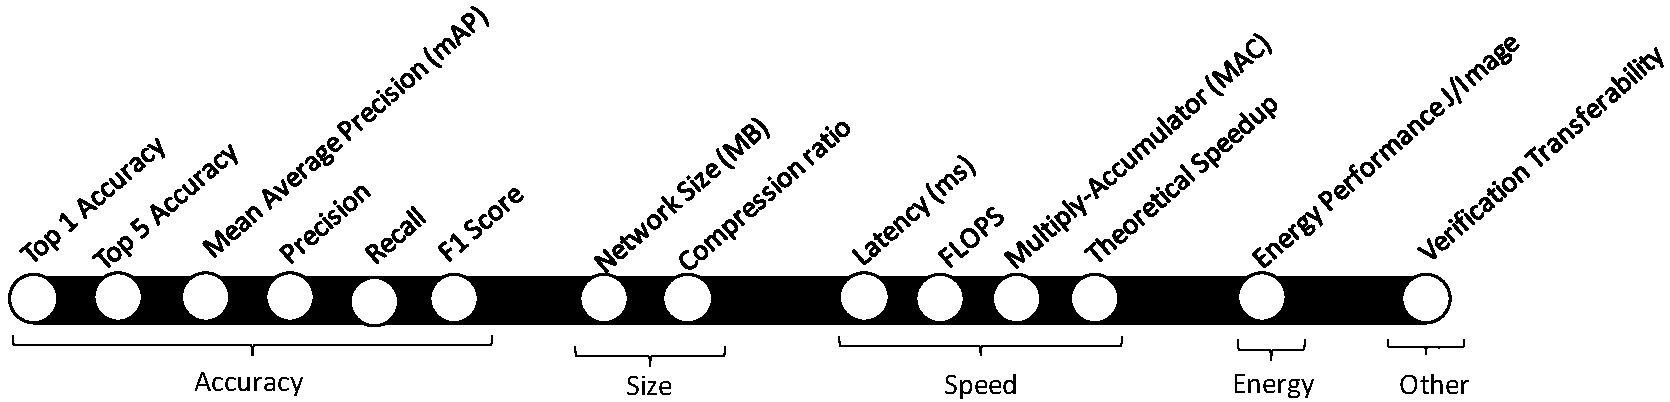
\includegraphics[width=1\textwidth]{figures/metrics.pdf}{}
%     \caption{Metrics}
%     \label{fig:metrics}
% \end{figure*}

In this section we cover a high-level overview of compression methods and we discuss existing compression benchmarks.% and how NetZIP compliments and extends existing works.

\subsection{Compression Methods Overview}
Following Neill et.al.~\cite{Neill2020} and Marino et.al.~\cite{Marino2023} overviews, compression techniques can be broken into four categories shown in Figure~\ref{fig:compression_methods} and briefly explained below:
\begin{enumerate}
    \item \textit{Pruning:} Requires the scanning and removing of neurons and connections that does not have a significant influence on the output prediction of the neural network.

    \item \textit{Quantisation:} Aims at reducing the numerical representation of values in a neural network model, for example by converting values expressed in a neural network from single-precision 32-bit floating point (FP32) numbers to 8-bit integers (INT8) or even to binarised neural networks~\cite{BNNs,TNNs}.

    \item \textit{Knowledge Distillation:} Trains a large neural network (teacher model) on a dataset. Then a smaller neural network (student model) is trained on the same dataset whilst guided by the teacher model through transfer learning techniques to help the student model optimise achieving similar accuracy as the teacher model.

    \item \textit{Tensor Decomposition:} Involves the decomposition of large weight tensors by approximating them to additions and products of lower order tensors.
      
\end{enumerate}
% \subsubsection{Pruning}
% Involves scanning and removing of neurons and connections that does not have a significant influence on the accuracy performance of the neural network.

% \subsubsection{Quantisation}
% Aims at reducing the precision of numerical values in a neural network model, for example by converting values expressed in a neural network from single-precision 32-bit floating point (FP32) numbers to 8-bit integers.

% \subsubsection{Knowledge Distillation}
% Trains a large neural network (teacher model) on a dataset. Then a smaller neural network (student model) is trained on the same dataset whilst guided by the teacher model through transfer learning techniques to help the student model optimise achieving more or less the same performance as the teacher model. 

% \subsubsection{Tensor Decomposition} Involves the decomposition of large weight tensors by approximating them to additions and products of lower order tensors.



% ==== Useful notes that might be worth keeping =====
% Survey \cite{Gholami2022}, \cite{Liang2021}

% Useful link that provides tips on deployment after quantisation and what you need to be aware of: https://spell.ml/blog/pytorch-quantization-X8e7wBAAACIAHPhT

% Paper that mentions one should avoid quaantising the first and last layer in a DNN https://arxiv.org/pdf/1603.05279.pdf
% ===================================


\subsection{Compression Benchmarks}
Creating benchmarks for standardising neural network compression is currently a growing area of research. %
%
Microsoft Neural Network Intelligence (Microsoft NNI)~\cite{nni2021} is an open-source toolkit that helps users automate the optimization of deep learning models. It supports different deep learning frameworks mainly PyTorch and TensorFlow, allowing users to easily run experiments for optimising their models. 
%
One of the core parts of Microsoft NNI toolkit is model compression. They provide a growing library of compression techniques available in the literature, such as~\cite{courbariaux2016binarized, esser2020learned, yang2022oneshot, frankle2019lottery}, making it accessible and efficient for users to experiment using state of the art compression techniques. Microsoft NNI also provides a web-based dashboard to track and visualize the results of experiments.
%
However, the toolkit does not dive into standardisation nor provides a comprehensive set of metrics for standardising the evaluation of neural network compression.

Blalock et.al.\cite{Blalock2020} tried to solve the lack of neural network compression standardisation in the community for pruning methods by analysing a large number of literature and generated a catalog of common issues in comparisons between pruning algorithms.
%
This was summarised into a set of best practices to mitigate these issues. Using these best practices they implemented ShrinkBench, a standardised library for pruning neural networks. 
%
% In summary these best practices are summarised here: 1) start from the same initial model 2) Compare accuracy and theoretical speed up for the same compression ratio, as different compression ratios may result in which compression technique is best....  
%
For NetZIP, we focus on evaluation to give a holistic view showing the pros and cons between different compression categories and algorithms. 
%
We chose to create NetZIP independently instead of extending ShrinkBench with our suite of metrics, as it was more effort efficient to build NetZIP to be lenient to accept different compression methods and focused on evaluation, rather than reconstructing ShrinkBench to allow it to accept different compression categories other than pruning. 
%
We take into account the best practices summarised by Blalock et.al.\cite{Blalock2020} when carrying out our experiments using NetZIP, as many of their best practices are applicable regardless of the compression method.
%
% NetZIP is also a standardised compression benchmark but aimed at providing a comprehensive set of metrics for evaluating deep neural networks compression techniques. The need for such a tool standardising metrics for compression as been pointed out implicitly by Blalock et.al.\cite{Blalock2020}. 

Facebook research provides some relevant evaluation metrics for neural networks as part of their \textit{Slowfast}~\cite{fan2020pyslowfast} repository implementation. Whilst the metrics provided are not comprehensive for compression methods evaluation, it has provided some insight in the course of development of our paper.

An issue relevant to the context of our paper is the difficulty in generalising the removal of zeroed parameters from different pruned neural network architectures. For example, current implementations of pruning in PyTorch sets a value of zero to the pruned parameters but do not automatically remove the zeros from the network structure. 
%
% This is because removing structural parameters from a neural network can result in malfunctioning of the network and generated errors. 
% %
% Hence, removing the zeroed parameters currently rely on manually designing case-dependent schemes that do not generalize to different neural network architectures. 
% %
% Developing a method for generalising and automating the removal of these parameters is beyond the scope of our paper. 
% % but we use the sparsity level to provide an evaluation of the compression in size as will be discussed later in the paper. Removing the zeroed parameters is case-dependent, 
%
This is because most network operations are large matrix multiplications, which have been efficiently implemented in software to perform operations on fully connected graphs. Therefore removing connections, will often require custom software, unless done in a software aware way. This problem lies outside the scope of this work.  
%
We direct interested readers towards DepGraph~\cite{fang2023depgraph} which aims at generalising the the approach of removing pruned parameters invariant of the architecture. 
%


%
% However, not being able to remove the pruned parameters stops us from evaluating benefits on model size from compression after pruning. We suggest


% Another interesting related work is DepGraph~\cite{fang2023depgraph}, which dives into the issues uctural pruning enables model acceleration by removing structurally-grouped parameters from neural net- works. However, the parameter-grouping patterns vary widely across different models, making architecture- specific pruners, which rely on manually-designed grouping schemes, non-generalizable to new architectures. In this work, we study a highly-challenging yet barely-explored task, any structural pruning, to tackle general structural pruning of arbitrary architecture like CNNs, RNNs, GNNs and Transformers. The most prominent obstacle towards this goal lies in the structural coupling, which not only forces different layers to be pruned simultaneously, but also expects all removed parameters to be consistently unimpor- tant, thereby avoiding structural issues and significant per- formance degradation after pruning.



% Current implementations of pruning PyTorch only aims at zeroing the pruned parameters but does not remove these parameters from the tensors, therefore the actual size of the saved model does not decrease. Sparsity can be a representative of Compression ratio for pruning. However, efforts are currently being devoted into creating libraries that 


% \cite{Babaeizadeh2016} propose NoiseOut, a fully automated pruning algorithm based on the correlation between activations of neurons in the hidden layers.

% \cite{Zhou2019a}




% \cite{Yang2019}

% Larqx



\section{Metrics}\label{sec:metrics}
In this section we overview different assessment metrics that serve the evaluation of DNN models and compression techniques. For each metric we discuss how it can be computed and the information it provides for assessment. We break the evaluation metrics into five categories: Accuracy, Size, Speed, Energy, and Combined Measures.%; each category has different evaluation metrics (see Table~\ref{tab:metrics_summary}).

% \setlength{\arrayrulewidth}{0.1mm}
% \setlength{\tabcolsep}{2pt}
% \renewcommand{\arraystretch}{1.75}
% \begin{table*}[]
%     \centering
%     \begin{tabular}{| c | l l l l l |} 
%         \hline
%         Category &  &  & Metrics &  &    \\
%         \hline
%         Accuracy & Top-k Accuracy &  Precision & Recall & F1-Score & mAP \\ 
%         Size     & Disk Size &  Parameters Count & CPU usage & GPU usage &  \\  
%         Speed    & Inference Latency &  Number of Operations & MACs & FLOPs &   \\ 
%         Energy   & Power &  Energy &  &  &  \\ 
%         Combined Measures    & Compression Ratio & Speedup Ratio &  Efficiency Ratio &  & \\ 
%         \hline
%     \end{tabular}
%     \caption{Metrics Summary}
%     \label{tab:metrics_summary}
% \end{table*}

\subsection{Accuracy}
In this section we discuss different metrics for measuring accuracy for both object classification and object detection.
%
We use true positives (TP) to refer to predictions that agree with ground truth; false positives (FP) for predictions which are considered false; and false negatives (FN) for ground truth annotations that were not detected.
%
In the context of object classifications, TPs are counted by simply matching the predicted label with the ground truth label. 
%
In object detection, a given bounding box is considered TP if the intersection over union (IoU), which is the ratio of overlap between a detected box and ground truth, is over a certain threshold.

% \subsubsection{Classification}
% Top-k accuracy measures the proportion of samples where the ground truth class is contained in the top-k predictions of a model~\cite{petersen2022differentiable}. Higher k is used when the number of classes is large and there are understandable confusions between some classes. 
\subsubsection{Top-k Accuracy}
% Top-k accuracy is used to measure the accuracy of a model.%, often used in the context of object classification.
%
Measures the proportion of samples where the ground truth class is contained in the top-k predictions of a model~\cite{petersen2022differentiable}, 
%
% Top-k accuracy shows the proportion of test samples for which the most likely $k$ predicted class labels match the ground truth class label
where $k \in \{1, ...,  K\}$ and $K$ is the max number of classes in the model being evaluated.
%
Two commonly used values for $k$ are 1 and 5. Top-1 accuracy in this case will only consider a prediction correct if it matches the ground truth label, whilst Top-5 accuracy will consider a prediction correct if one of the top 5 predictions of the model output matches the ground truth label. 
%
Top-k accuracy, for $k>1$, can be particularly useful where the model has a large number of classes, with several classes being similar to each other or where understandable confusions exist between some classes. %between them. 
%
In this case it may be challenging for the model to accurately predict the correct class, but for example a prediction amongst the top three possibilities may still be helpful.





% Detection:
% * IoU: For detection a given bounding box is considered true if the IoU (the measure of ratio of overlap between a detected box and ground truth) is over a certain threshold (normally 0.5).
% * TP: Detections which are considered true. 
% * FP - Detections which are considered false.
% *FN - Ground truth that was not detected.
% * Precision - the portion of detections that are TPs. [equation]
% * Recall - the portion of ground truth that were detected [ equation]
% * F1 Score - [ keep yours]
% * MaP - [keep yours]

% I question your choice of F1 score - i.e. picking a single threshold, it does not give a fair caparison and could lead to misleading results if a compression technique is threshold sensitive. I appreciate you may not have time to change this.



\subsubsection{Precision}
% Precision is a measure of the accuracy of the predictions output by a model, which aims at conveying how many of the predictions are accurate out of all predictions. 
%
% In other words, 
Is the the portion of predictions that are TPs, see equation~\ref{eq:precision}. 
%
% In object detection, given a bounding box the intersection over union (IoU) is calculated as the ratio of overlap between the ground truth annotations and the output predictions. If the IoU passes a certain chosen threshold, then the prediction is counted as TP. 
\begin{equation}
  Precision =   \frac{TP}{TP+FP}
  \label{eq:precision}
\end{equation}

\subsubsection{Recall} Is the portion of ground truth annotations that were predicted by the model, see equation~\ref{eq:recall}.
% is a measure that expresses the rate of a model getting correct predictions.
% Is a measure of how well a model is able to identify all instances of a particular object class within an image or a set of images.
%
% Specifically, recall is the fraction of true positive predictions, out of all present instances in the test sample  i.e. true positives + false negatives (FN), see equation~\ref{eq:recall}.
%
% Recall is an important measure in object detection, as it helps to ensure that a model is not missing any instances of a particular object class. However, it should be used in conjunction with other metrics, such as precision and mean average precision (mAP), to provide a more complete evaluation of the performance of an object detection model.

\begin{equation}
  Recall =   \frac{TP}{TP+FN}
  \label{eq:recall}
\end{equation}

\subsubsection{F1 Score} Is a metric that combines both precision and recall into a single metric. The F1 score is the harmonic mean of precision and recall, given by equation~\ref{F1_score}.
%
The F1 score provides a way to balance the trade-off between precision and recall, as both measures are important for different aspects of model performance. A high F1 score indicates that a model has both high precision and high recall%, meaning that it is able to correctly identify a high percentage of positive instances whilst also minimizing the number of false positives.

\begin{equation}
  \text{F1 Score} =   \frac{2 \cdot \text{Precision} \cdot \text{Recall}}{\text{Precision} + \text{Recall}}
  \label{F1_score}
\end{equation}

\subsubsection{Mean average precision (mAP)} Is a metric that takes into account both precision and recall of a model. 
%
The metric is calculated by summing the average precision ($AP$) of each class $k$ over the number of classes $K$, as shown by equation~\ref{eq:mAP}.  
% of the the mean of the different average precision for different classes as shown by equation~\ref{eq:mAP}
%
The AP of each class is calculated by plotting precision for different recall values and calculating the area under the curve (AUC)\footnote{To plot the precision-recall graph an IoU threshold needs to be selected. In the case where an optimal IoU threshold is not selected or unknown, then the AUC can be calculated for several IoU thresholds and averaged to give an AP representative of a range of IoU thresholds.}.
%
Compared to F1 score, mAP is more sensitive to imbalances in the number of training samples between different classes, whilst the F1 score is insensitive to these imbalances in training samples. On the other hand mAP is more expensive to compute compared to the F1 score.
%
% When the model is at the stage of training, mAP is a more informative metric to use in assessing the performance of the model on different prediction classes. 
% %
% However, in comparing between compression techniques the F1 score may be a more efficient metric for carrying out an initial assessment to identify best compression techniques. Dependent on application, analysis using mAP may still be useful.

\begin{equation}
    mAP = \frac{1}{K} \sum_{k=1}^{k=K} AP_k
    \label{eq:mAP}
\end{equation}

\subsection{Speed}
\subsubsection{Inference Latency} Is the time taken for the model to output its prediction. 
%
Whilst inference latency may give the most practical real-time value for operational speed estimates and machine specific comparisons, it is affected by resource utilisation at the time of measurement. 
%
This makes the measured inference latency variant to the level of resource utilisation, thus can be less informative about the benefit of compression in some cases. Especially if experiments are run on different machines or at different times where the level of resource utilisation may vary. 
%
This is analogous to an issue in simulation based testing, where variances in results for the same test can vary significantly due to resource utilisation changes~\cite{determinisim}.
% %
% In cases where the resource utilisation is known to have significant variations, one may resort to counting the number of operations or analysing the different proportions of numerical representation in the model after compression to deduce signs of speed improvement.
% %
% These other metrics may be useful when comparing between different compression algorithms within the same category of compression (e.g. pruning only or quantisation only) but may suffer from providing useful information when comparing between different compression categories. 
% %
% This is discussed further below, however, during carrying out our experimentation, we found that controlling the resource utilisation and using inference latency as a metric is the best way to quantitatively compare improvements in speed between different compression categories.


\subsubsection{Number of Operations (OPs)}
The number of operations (OPs) required to process a given input, can provide a hardware agnostic measure of the improvement in speed gained by a compression method.
%
It does not provide any information for quantization as this family of compression does not reduce the number of OPs, just the amount of hardware needed to carry out a given operation~\cite{Budgett2022}. 
%
% If a given quantisation is supported by the hardware for most neural network operations the hardware requirement scales as the square of the number of bits. 
%
Floating point operations (FLOPs) are often referred to in literature instead of OPs due to most neural network processing being done with floating point operations. However, here to generalise between floating point and quantised operations we will use OPs.
%
Furthermore, most operations in a neural network are multiply-accumulator operations (MACs), which contain one multiplication and one addition operations. Therefore a neural network typically has half the MACs compared to OPs. Given that MACs refer to the majority of neural network operations and some hardware are tuned to processing MACs, this measure is often used instead of OPs.  


% ====================================

% Computing the total number of operations for a neural network to output a prediction can be another way of measuring the improvement in speed gained by compression. 
% %
% This is especially useful when carrying out experiments on different machines or if resource utilisation varies between different experiments run on the same machine. 
% %
% For quantisation techniques, however, only the numerical representation type changes in the neural network but the number of parameters stay the same in the model. 
% %
% Even though quantisation does provide improvement in speed, calculating the number of operations may not provide any insight of that, as the number of operations count will be the same pre- and post-compression. 
% %
% For other compression techniques like pruning for example where parameters are removed from the model, measuring the number of operations can be an insightful metric for evaluating speed improvements.

% Floating-Point Operations (FLOPs) is a popular metric in measuring the speed improvement in compression literature especially for pruning. FLOPs only takes into account floating points operations. 
%
% Therefore, for quantisation techniques where the parameters are not of type float, not all operations will be counted. This may convey inaccurate estimations of speed improvements when comparing between quantisation and pruning techniques. Nevertheless, observing proportions of different types of numerical representations may give insights of speed improvements.  

% Multiply-Accumulator Operations (MACs) is another commonly used metric to count operations that involve all types of numerical representations i.e. not only floats. There are not any obvious advantages, as far as we are aware, of using MACs over the total number of operations referred to earlier. Perhaps the main strength of using MACs is its popularity over total number of operations. One MAC is defined as containing one multiplication and one addition operations, therefore MACs can be calculated as the total number of operations divided by two. 

\subsubsection{Compression and Hardware Agnostic Theoretical Speed (CHATS)}
Given the current limitations of previously discussed speed metrics, relating to poor generalisation between compression techniques and sensitivity to resource utilisation variances, we introduce the \textit{CHATS} metric.
%
CHATS aims at providing a theoretical speed quantity that is agnostic to the compression technique, and simultaneously not affected by the resource utilisation levels of hardware.
%
The metric succeeds in providing such theoretical speed by combining OPs with the bit width representation used by the model, see equation~\ref{eq:CHATS}.

The number of binary digits to be processed scales as the square of the bit width for multiplication, whilst for addition it scales linearly with the bit width. 
%
In DNNs, where both multiplication and addition may exist, the actual reduction in processing binary digits as a result of reducing the bit width will scale somewhere between the square of the bit width and linearly with the bit width. 
%
Leading GPU developers such as NVIDIA, often report improvements in theoretical speeds as a linear relationship with bit width e.g.~\cite{NVIDIA_TURING_GPU_ARCHITECTURE_2018}.  
%
Similarly, we also adopt a linear relationship with bit width when calculating CHATS. We introduce a hardware specific constant, $\zeta$, when calculating the speedup ratio for CHATS (see section~\ref{combined_measures}) to act as a scaling coefficient dependent on the hardware. 
%
For example, for results of NVIDIA Turing Tensor Cores hardware shown in~\cite{NVIDIA_TURING_GPU_ARCHITECTURE_2018}, the speedup ratio scales linearly with the bit width and hardware constant $\zeta = 4$. 

Furthermore, as technology of DNNs tailored hardware advances to prioritise efficiency, where multiplication operations dominate~ e.g.~\cite{Budgett2022}, we may find that CHATS scales as the square of the bit width. Investigating this further remains as future work. 



% For tailored hardware to the bit width, we speculate that this relationship scale as the square of the bit width instead.
 
%
% Based on empirical results provided by Budgett and deWard~\cite{Budgett2022}, they report that the square of the bit width gives roughly the hardware scaling required. 

\begin{equation}
    CHATS = OPs \cdot bit width
    \label{eq:CHATS}
\end{equation}

\subsection{Size}
\subsubsection{Disk size}
The space required to keep the model on a computer can be of significance especially when models are large e.g. ChatGPT-3~\cite{Brown2020}. Compression techniques can help in significantly reducing the model size so less disk space is required. For example quantisation of model parameters from FP32 to INT8 numerical representation decreases disk size required to save the model typically by a quarter. 
%



% - discuss point on sparsity here as well

 

\subsubsection{Parameters Count}
Another way of measuring the size of the model is by counting the number of parameters in the compressed model compared to the uncompressed version. This method can be useful when comparing compression techniques where parameters are actually removed from the model e.g. pruning. 
%
The usefulness of parameters count will fall short when it comes to quantisation techniques, where the number of parameters stay the same but the numerical representation changes.
In these cases using the disk size as a metric to compare between compression techniques can be a more informative measure than parameters count.
%
Nevertheless parameters count can be of great use at early stage assessment of pruning techniques.
%
In many of the popular pruning libraries implementations e.g. PyTorch~\cite{paszke2017automatic}, typically the pruned parameters are zeroed but not removed from the model.
%
% This is due to errors likely to occur when structural parameters are removed in pruning. Removing the zeroed parameters from the architecture is currently an active area of research e.g.~\cite{fang2023depgraph}, as currently removing the pruned parameters is a manual and custom process reliant on the model architecture. 
%
Therefore, non-zeroed parameters count can serve to show how much reduction in disk size will be achieved using different pruning techniques, prior to committing to the manual process of removing pruned parameters. 
%
Furthermore, the proportion of the uncompressed model parameters which are zeros after compression is known as \textit{sparsity}.
% ratio of zeroed parameters over the tota metric derivative of parameters count showing what 
% Note: Due to errors likely to occur when structural parameters are removed inp pruning as discussed earlier in our related work section, we use the sparsity in the neural network to measure the size/compression ratio.


% \subsubsection{Space and Resource Theroitcial Size (SARTS)}
% Params . bit . 

\subsubsection{CPU/GPU utilisation}

When CPU is not running a program, it is \textit{idle}. The running total (RT) is the total time the CPU spent on running programs i.e. not being idle, through out the switched on time of the computer. 
%
The CPU utilisation is the percentage of time the CPU is not idle, calculated by subtracting two samples of RT and dividing by the time between taking the two samples.
%
Figure~\ref{fig:cpu_utilisation_illustration}, shows an illustration for CPU switching between running a program and being idle. If sample measurements are taken every five seconds, then the CPU utilisation for the initial 5s was 60\% then dropped to 40\%. 
%
GPU utilisation will take  a similar approach of measuring time spent on processing requests against idle time to calculate utilisation. 
%
In terms of how CPU and GPU utilisation can be measured practically, \texttt{psutil} \cite{psutil2019} and \texttt{nvidia-smi}~\cite{NVIDIA_SMI} are popular libraries that provide these measurements.

Measuring the reduction in computational resources used by the model to output a prediction is an important factor to assess when investigating the trade-offs between different compression techniques.
%
When taking measurements for utilisation, other programs should be terminated and only the model outputting predictions should be the running process. In most computers, however, there are many background processes that need to run for the computer to operate. 
%
In which case, the best estimate is to subtract the utilisation measurement before and during making predictions.

\begin{figure*}[h]
    \centering
    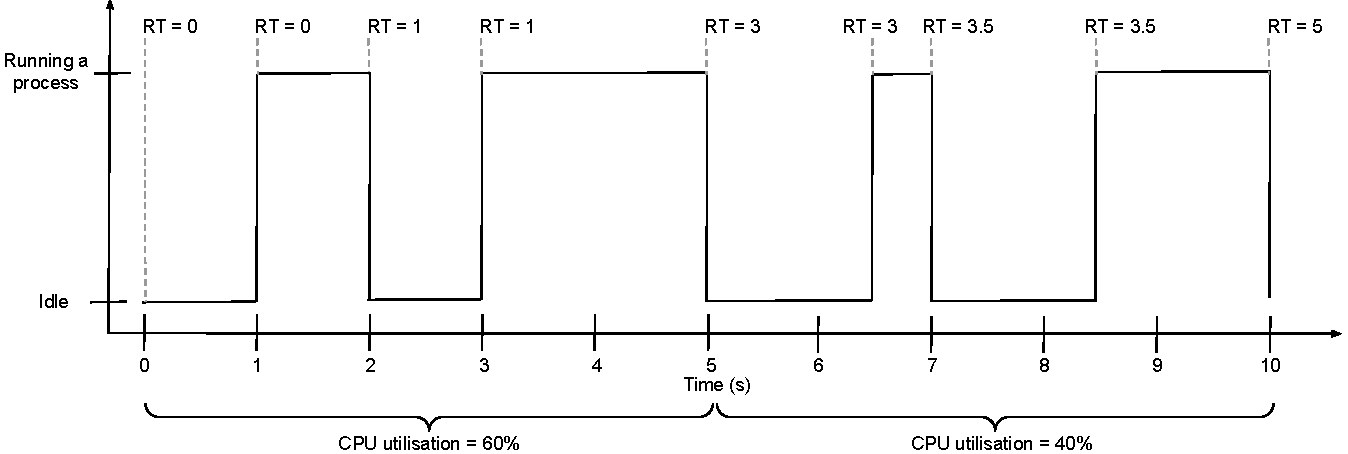
\includegraphics[width=0.8\textwidth]{other/figures/CPU_utilisation_diagram_v1.pdf}
    \caption{Illustration of CPU switching between running a process and being idle.}
    \label{fig:cpu_utilisation_illustration}
\end{figure*}

\subsubsection{RAM usage}
RAM (Random Access Memory) usage in inference is a measure of paramount importance to report. 
%
Knowing how much reduction in RAM usage is achieved by different compression techniques can be advantageous in determining specifications of hardware needed for a model to operate on SWaP devices.
%
Libraries such as \texttt{psutil} \cite{psutil2019} can be used to determined RAM usage.
%
Similar to CPU utilisation, when taking measurements of RAM usage, other programs should be terminated other than the inference model. 
% Also subtracting RAM usage before inference from usage during inference give the best estimate 
%
% In which case, the best estimate is to subtract the utilisation measurement before and during making predictions.

% Measuring CPU and even GPU useage can be achevied ....

% ========================

% The two types memory of most relevance for neural network compression evaluation are, random-access memory (RAM) and storage memory such as hard disk drives (HDDs) and solid-state drives (SSDs).
% %
% RAM is used to store data and instructions that the computer is currently using. 
% %
% Storage devices such as hard disk drives (HDDs) and solid-state drives (SSDs) are used to store data and programs over a long period of time, even when computers are turned off. 
% %
% Therefore, for evaluating DNNs compression there are two metrics identified for evaluating \textit{size}:

% \subsubsection{RAM utilisation}
% There may be various ways of measuring RAM utilisation, however, since NetZIP is based on python and implemented in Linux, we use the {\tt psutil} python library. 

% \subsubsection{Storage size}
% To measure the size of the stored file we use the built-in python library os function {\tt os.path.getsize()}.




\subsection{Energy consumption}
Energy consumption can be calculated by plotting power against time and the area under the plotted curve is the energy consumed.
%
In other words, energy consumed $E$ is the integration of power $P(t)$ as function of time $t$ over the duration $t_0$ to $T$, given by Equation~\ref{eq:energy}.

\begin{equation}
    E = \int_{t_0}^{T} P(t) \,dt = \sum_{t=t_0}^{t=T} P(t)\cdot  dt
    \label{eq:energy}
\end{equation}

Figure~\ref{fig:energy_illustration} illustrates the measurement of energy consumption using fine and coarse sampling rates of power. It is important that sampled power measurements are fine enough to sufficiently capture detail in the energy consumption profile. For example as illustrated by the right diagram in Figure~\ref{fig:energy_illustration} a spike in the energy consumption profile was missed due to the coarse power reading intervals.
% spike energy consumption measurements will miss spikes in energy consumption as shown by the right diagram in Figure~\ref{fig:energy_illustration}.

Measuring the energy consumption of a neural network depends on various factors such as the hardware platform and the workload being executed. 
%
For reliable comparisons of energy consumption one need to ensure that the same hardware is used and the same resource utilisation setting.
%
One common python library used to measure energy consumption in computers employing Intel processors is pyRAPL, which is a python toolkit used to measure the energy footprint of the CPU~\cite{pyRAPL_repo}.  
%
Whilst pyRAPL may give good indicative estimates of energy consumption, its measurements are reliant on estimation models instead of live measurements of power. 
%
This may be useful for trying to improve the energy utilisation of a machine but may fail when it comes to budgeting for energy requirements, which is critical in some application e.g. space applications.
%
Using pyRAPL also limits measurement to hardware only employing Intel processors. 

%
A more generic  way is to use power measurement tools that can connect between the power source and the hardware platform to measure the power consumption in real time.%~\cite{any references from Kerstin's previous energy works}. 
%
This way of measuring energy is more informative for applications requiring energy budgeting. 

\begin{figure*}[h]
    \centering
    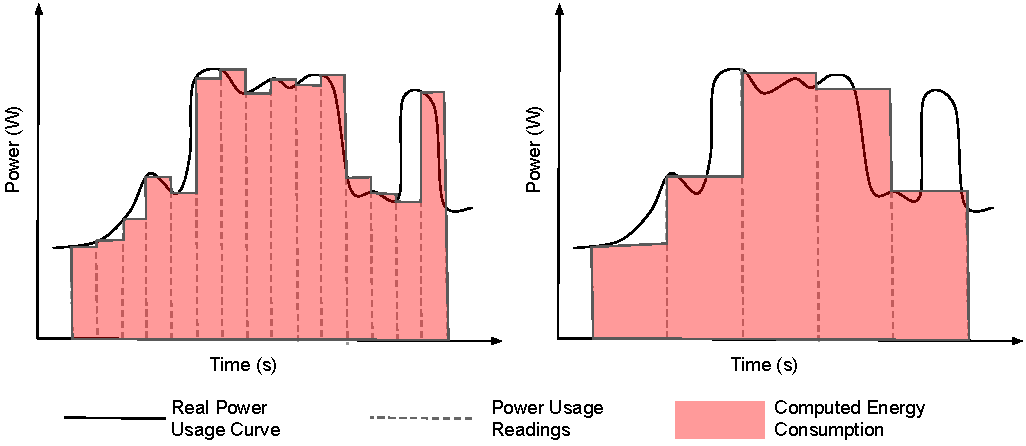
\includegraphics[width=0.6\textwidth]{other/figures/energy_measurment_schematic.pdf}
    \caption{Illustration of energy measurement from fine (left plot) and coarse (right plot) power reading intervals.}
    \label{fig:energy_illustration}
\end{figure*}

\subsection{Combined Measures} \label{combined_measures}
We use this section to capture derived metrics from the aforementioned metrics.% and discuss potential future metrics that can benefit the evaluation of compression techniques. 
%
% \subsubsection{Improvement Ratio}
It is often that improvement ratio provided by a compression technique is reported in the literature ~\cite{He2018,Blalock2018,Menghani2023}. Two popular improvement ratios are \textit{compression ratio} and \textit{(theoretical) speedup ratio}.
%, given by equations \ref{compression_ratio} and \ref{speedup_ratio} respectively.
%
The speedup ratio refers to the reduction in computation time that can be achieved by using a compressed model, relative to the original uncompressed model. Typically calculated as a ratio between the computation time of the uncompressed model and the computation time of the compressed model (see Equation~\ref{speedup_ratio}). When this speedup ratio computation is carried out using a non temporal metric e.g.(OPs, FLOPs, MAC) then it is referred to as \textit{theoretical speedup}. 
We incorporate a hardware specific constant, $\zeta$, in the speedup ratio to provide means of correcting the speedup ratio based on the operational hardware. %For example, for results of throughput discussed in \cite{NVIDIA_TURING_GPU_ARCHITECTURE_2018},  $\zeta = 4$   

%
% \subsubsection{Compression Ratio}
\textit{Compression ratio} is another derived metric based on size reduction of the model. It refers to the reduction in model size achieved by a compression technique, relative to the size of the original uncompressed model (see Equation~\ref{compression_ratio}). 
%
We extend this further to include \textit{efficiency ratio} (Equation~\ref{effeciency_ratio}) and \textit{performance ratio} (Equation~\ref{performance_ratio}), which aim at reporting improvements in  energy consumption and accuracy, respectively, between the compressed and uncompressed models.


\begin{equation}
  \text{Speedup ratio} =   \zeta \cdot\frac{\text{original speed}}{\text{compressed speed}}
  \label{speedup_ratio}
\end{equation}

\begin{equation}
  \text{Compression Ratio} =   \frac{\text{original size}}{\text{compressed size}}
  \label{compression_ratio}
\end{equation}

\begin{equation}
  \text{Efficiency Ratio} =   \frac{\text{original energy consumption}}{\text{compressed energy consumption}}
  \label{effeciency_ratio}
\end{equation}

\begin{equation}
  \text{Performance Ratio} =   \frac{\text{compressed accuracy}}{\text{original accuracy}}
  \label{performance_ratio}
\end{equation}

Reporting improvement ratios alone is not enough, as the ratio can be calculated using different metrics, for example one may calculate the compression ratio using disk size, whilst another can use parameters count, or CPU/GPU usage to calculate the compression ratio. Similarly, one may use inference latency, OPs, or MAC to compute speedup ratio.
%
Therefore when reporting improvement ratios, one need to outline what metrics were used in their computation to allow for reliable comparisons between different works.

\subsubsection{Overall Compression Success (OCS)}
We introduce the Overall Compression Success (OCS) metric. The metric combines the different improvement ratios into one metric summarising the overall success of a compression technique. 
%
OCS is shown by equation~\ref{OCS}, where P, S, C and E are the calculated performance, speed, compression and efficiency ratios respectively. 
%
The $\lambda$s are weight parameters, to allow for adjusting the importance of the different assessment categories. 
%
The OCS metric is set in a way to output a positive value if there is an overall improvement, a negative value if there is an overall  worsening. OCS will output a value close to zero if there is no change from the uncompressed model, the trade-offs cancel out, or the compressed model accuracy has dropped significantly. 

\begin{equation}
  \text{OCS} =  P \cdot \Bigl( \lambda_1 (P-1) + \lambda_2 (S-1) + \lambda_3 (C-1) + \lambda_4 (E-1) \Bigl) 
  \label{OCS}
\end{equation}

\section{NetZIP Overview} \label{sec:NetZIP_overview}
% \subsection{Overview}
% We have put together a library containing all of the metrics reviewed in this paper and named it NetZIP. NetZIP 
%
We introduce NetZIP, a library based on PyTorch~\cite{paszke2017automatic} that provides a suite of metrics for evaluating the gains and losses in performance from different compression techniques.
%
The suite of metrics is based on the five evaluation categories reviewed in  section~\ref{sec:metrics}.
%
The goal of NetZIP is to provide a unified implementation of assessment metrics to ease and standardise the evaluation of compression techniques. Allowing for more reliable and unified comparisons across works by different researchers.
%
We provide a set of datasets and models to be used as baselines for running experiments, and help researchers get started.  
%
The NetZIP library may improve and and grow overtime, to include more baseline experiment and more metrics as research on neural network compression evolves. 
%
Figure~\ref{fig:Netzip} depicts an overview diagram of NetZIP showing how users may utilise NetZIP for their evaluation setup. 
%
Following lessons learnt from Blalock et.al.~\cite{Blalock2020}, one should compare models that have been compressed from the same uncompressed model; therefore we break NetZIP into three main stages: Train, Compress, and Compare. 

Using NetZIP, one can train a model from scratch or use a pretrained model and extend its training. 
%
The trained model is saved, and then in the ``Compress" stage this saved model is used as the starting uncompressed model for every different compression technique used. 
%
One can either use baseline compression methods available or program their own custom compression technique that they wish to evaluate. The different compressed models are saved and can be evaluated in the ``Compare" stage. 
%
In the ``Compare" stage, the user can select several options from the metrics suite to evaluate the compressed models against the uncompressed model and output a summary log file along with plots for each metric.% comparing the different compression techniques.% for each selected metric.
%
% Whilst one may utilise the ``Compare" stage in NetZIP to compare readily compressed models, we recommend to use the workflow constructed in the NetZIP library shown in Figure~\ref{fig:Netzip}, to ensure that any gains you get from compression is due to the compression technique used and not due to the different training or configuration settings.


\begin{figure*}[h]
    \centering
    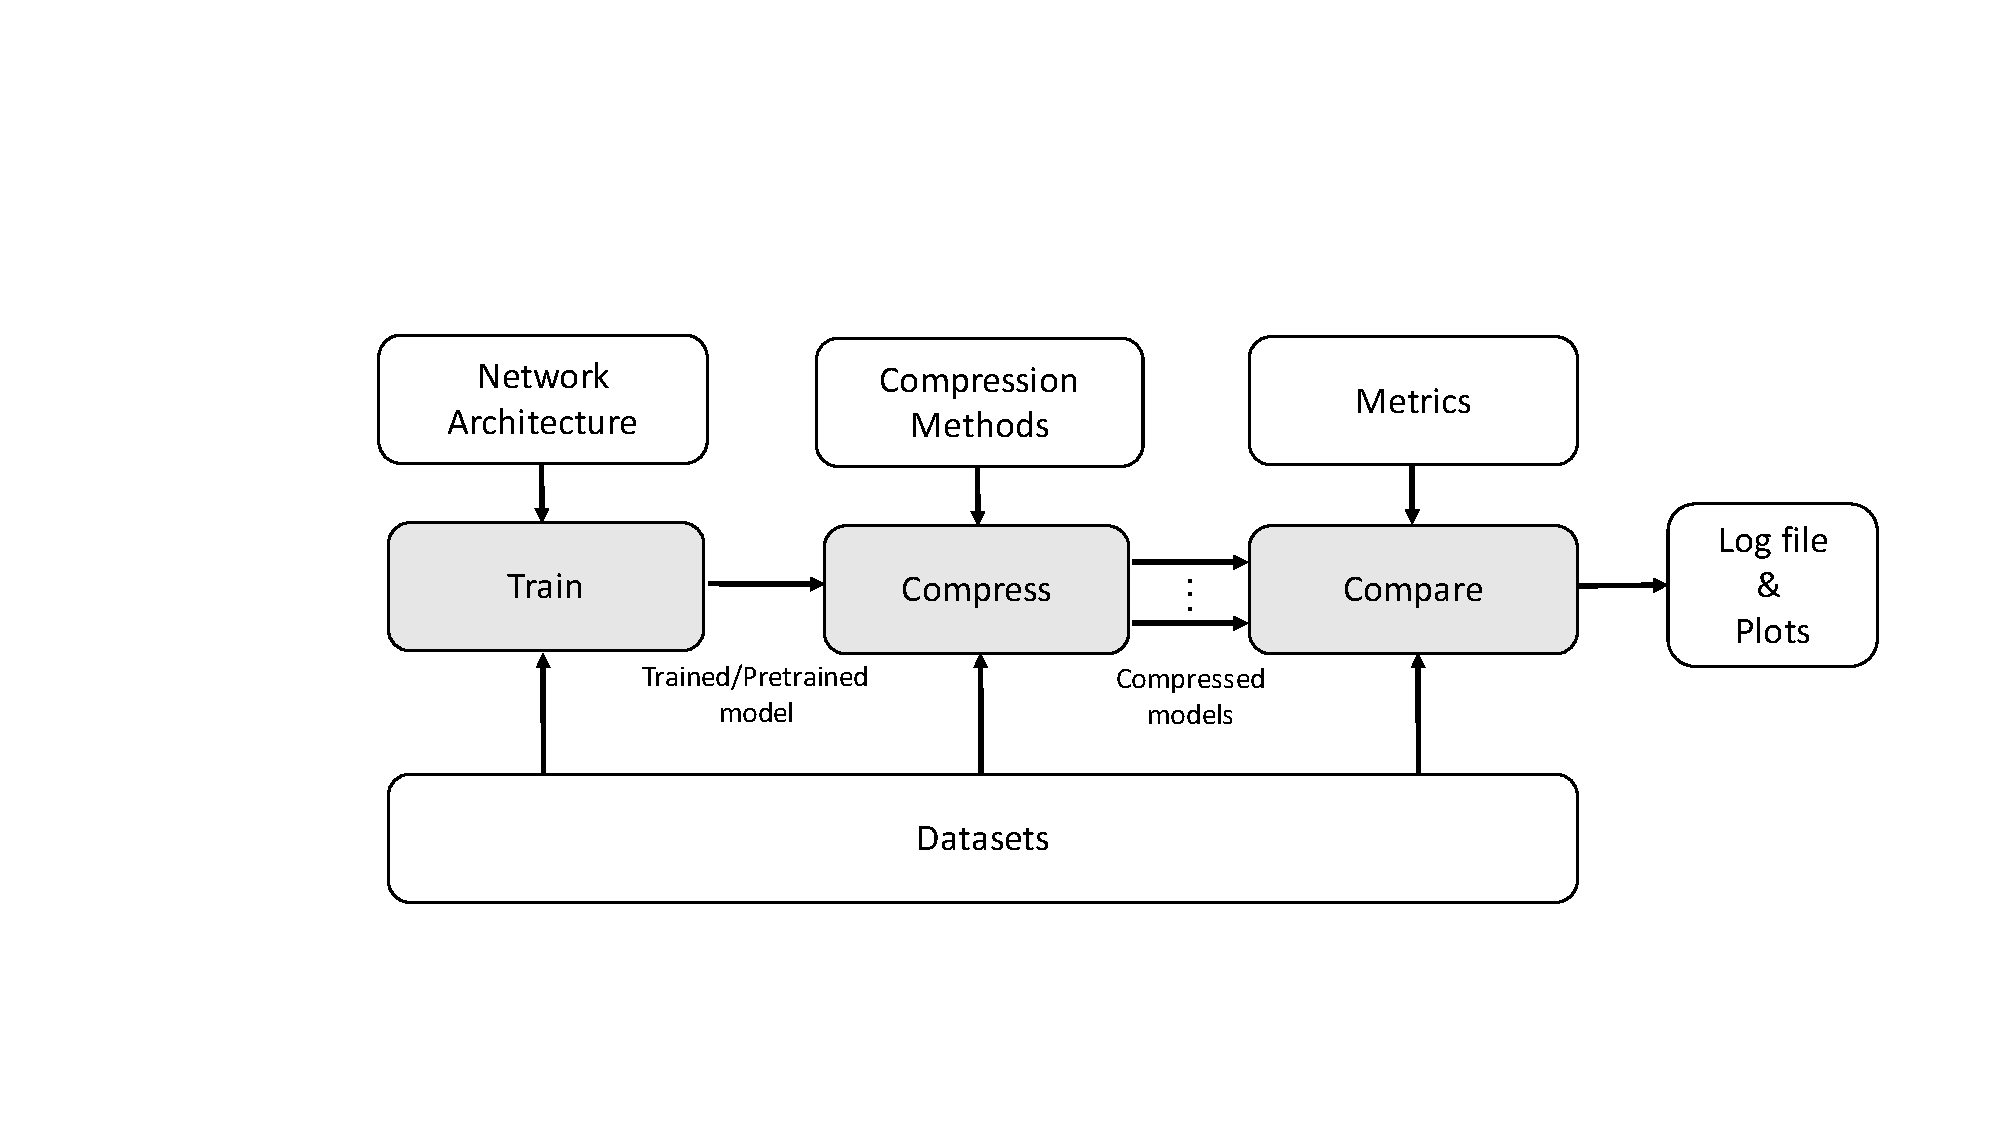
\includegraphics[width=0.7\textwidth]{other/figures/NetZIP_overview.pdf}
    \caption{NetZIP overview}
    \label{fig:Netzip}
\end{figure*}



\section{Example Case Studies} \label{sec:casestudies}
We use two case studies implemented as part of NetZIP, to showcase some of the evaluation metrics reviewed and the novel metrics we contributed in this paper. 
%
Table~\ref{tab:casestudy_summary}, shows a summary of the two case studies, including the neural network architectures, datasets, compression techniques, and the hardware used in our case studies.
%
Table~\ref{tab:Hardware_summary} shows the hardware specifications. 
%
In all of our evaluations we eliminated the usage of GPU and used only CPU, to maintain fair availability of resources in our experiments, especially that some compression techniques implementations currently only operate on CPU. 
%
The majority of metrics used in the assessment are the same for the both case studies, as can be seen from the results tables~\ref{tab:resnet-imagnet1k} and ~\ref{tab:Yolov5s-COCO}. The only different assessment metric is the accuracy metric, for case study 1 we used top-1 accuracy and for case study 2 we used mean average precision.

\subsection{Case Study 1}
In the first case study we selected object classification as our theme, using ResNet18~\cite{he2015deep} architecture on ImageNet1k~\cite{imagenet_cvpr09} dataset. This case study was run on a power full Dell Alienware PC with 64 GB of RAM.
%
We used four compression techniques available in the 
 PyTorch library, two based on quantisation and two based on pruning: 
\begin{enumerate}
    \item Post Training Quantisation (PTQ), where the model is trained on the dataset and then quantised.
    
    \item Quantisation Aware Training (QAT), where the model is trained on the dataset, quantised and then further training is done to try and recover drop in accuracy as result of quantisation.

    \item Global Unstructured Random Pruning (GUP$_R$), where parameters through out the model are pruned randomly until the required level of sparsity is achieved. 

    \item Global Unstructured L1-norm Pruning (GUP$_{L1}$), prunes the least significant parameters in the model globally until the required level of sparsity is achieved. 
\end{enumerate}

\subsection{Case Study 2}
The second case study focuses on object detection using YOLOv5s~\cite{Jocher_YOLOv5_by_Ultralytics_2020} to output predicts for COCO~\cite{lin2015microsoft} dataset.
%
We use the compression methods already integrated within the YOLOv5 repository~\cite{Jocher_YOLOv5_by_Ultralytics_2020}, which are limited to post training quantisation using TensorFlow lite (PTQ-TFlite) to FP16 and INT8 numerical representations. We also included in our comparison the Tensorflow (TF) FP32 version of the YOLOv5s architecture. 
%
In this case study we have run experiments using Raspberry Pi 4 Moodel B, as means of studying benefits of compression on hardware with limited resources.

\begin{table*}[]
    \centering
    \begin{tabular}{| c | c  | c | c | c | c |} 
        \hline
        Case Study No. & Theme & Network Architecture & Datasets & Compression Techniques & Hardware  \\
        \hline        
        1 & Object Classification  & ResNet18 & ImageNet1k & PTQ, QAT, GUP$_R$, GUP$_{L1}$ & PC \\ 
        % Object Detection  & YOLOv5s & COCO  &  PTQ-TF  & Laptop  \\
        2 & Object Detection  & YOLOv5s & COCO  & PTQ-TFlite  & RasPi 4 \\
        \hline
    \end{tabular}
    \caption{Case Studies Summary}
    \label{tab:casestudy_summary}
\end{table*}
%
\begin{table*}[]
    \centering
    \begin{tabular}{| l  | l | l | l |} 
        \hline
        Name & Product Name & Specifications & Operating System \\
        \hline        
        % Laptop  & MSI GF65 THIN 3060  & 64GB RAM%, NVIDIA 3060 & Linux Ubuntu 20.04.2 LTS (64-bit)\\ 
        PC  & Dell Alienware Desktop & 64GB RAM%, NVIDIA 2080 
        & Linux Ubuntu 18.04.4 LTS (64-bit)\\
        RasPi 4  & Raspberry Pi 4 Model B & 4GB RAM &  Linux Ubuntu 22.04.2 LTS (64-bit) \\
        \hline
    \end{tabular}
    \caption{Hardware Specifications Summary.}
    \label{tab:Hardware_summary}
\end{table*}


\section{Results and Discussion}

% == Tables results
Tables~\ref{tab:resnet-imagnet1k} and ~\ref{tab:Yolov5s-COCO} shows results for case studies 1 and 2 respectively. 
% Changes in Accuracy
For case study 1 , the accuracy of PTQ provided the least drop in accuracy of 0.2\% compared to the uncompressed model,  whilst GUP$_R$ had the most significant drop in accuracy of about 19.5\%. 
%
In the second case study, there were no significant drops in accuracy, the highest drop of 1.9\% was incurred by PTQ TFlite (INT8) compression technique.   

% Speed gains. Using latency. 
In terms of speed, compression provided improvements in both case studies.  
%
For the first case study compressing using quantisation improved the inference latency by $\times 2$. However, no changes in speed are seen for pruning techniques.
%
Noting that monitoring inference latency is sensitive to hardware resource utilisation, we resort to observe the MACs metric, which is insensitive to resource utilisation variations. 
% Using MACS and CHATS.
MACs suggests there should be no change in speed for any of the compression techniques, but using the CHATS metric we introduced, it can be seen that it suggests that inference time should decrease for quantisation techniques but should stay the same for pruning techniques.
% Pruning limitations
As discussed previously in our related works section, current implementations of pruning are limited to setting pruned parameters to zero but they are not actually removed from the model. Therefore, we see changes in accuracy due to pruning, but not in speed or any of the other metrics. 
% Hence, the current results for pruning compression techniques are not expressive of the benefits from pruning. 
%
% TF model perfomraning better than compressed models.
For the second case study, the latency and CHATS decreased as expected, with increasing quantisation levels. 
%
However, interestingly the TensorFlow FP32 model had the least inference latency.  
%
We speculate that this may be a result of different library implementations compared to PyTorch. 
%
Investigating these speculations are beyond the scope of this paper, however it is important that these factors are investigated further in real life applications.
%
Using CHATS as a metric for comparing between compression techniques can be a more reliable metric to use in such cases.

In both case studies compression using quantisation decreased the disk size of the model but has not changed the parameters count as expected. 
%
For pruning in the first case study this decrease can not be noticed, but to showcase the potential provided by pruning in size reduction we have included the parameters count for non zero parameters between brackets.
%
% Gains in Hardware utilsiation
Reducing hardware usage by compression was not observed in neither CPU utilisation nor gigabytes of RAM usage for case study 1.
%
On the other hand, on less powerful hardware used in case study 2, significant reduction in hardware usage can be observed for compressed models.

% Gains in Energy utilisation
Last but not least compression had energy consumption improvements in both case studies. The interesting observation is in case study 2, that is even though the TF (FP32) implementation had better speed compared to TFlite (INT8), the energy efficiency of the PTQ TFlite (INT8) was best.  
%
This observation is very interesting as one may expect the INT8 implementation to be both quicker and more energy efficient. 
%
Field et.al.~\cite{Field2014} reported a similar observation, where shorter bits save more energy but take more execution time than longer bit representations. 
%
This may perhaps be resolved through reconfiguration of hardware, however, it is beyond the scope of this paper to investigate technically how this can be achieved.

% == Improvement Ratios 
Furthermore, as can be seen comparing benefits of compression is multivariate, which can be difficult to quickly digest when comparing different techniques. Here is where our overall compression success (OCS) metric can assist. It can give an overall idea of which techniques is best overall. This is more informative when viewed a long with the other improvement ratios. 
%
Therefore, we choose to view the overall compression success using spider web diagrams (or radar charts), which provides an optimal way for observing overall compression success and the trade-offs made (see figure~\ref{fig:Radar-spider}) in the different assessment categories. 
%
The OCS and each improvement ratio are represented by a separate axis in figure~\ref{fig:Radar-spider}. Data
points for each improvement ratio are plotted on the axes and connected to form a polygon. 
%
The value of OCS and the shape of this polygon represent a more tangible approach for assessing the best compression technique. 
%
Using the spider web diagrams in figure~\ref{fig:Radar-spider} it can be seen that in case study 1, PTQ and QAT both have equivalent overall compression successes, whilst in case study 2 the quantisation to TFlite INT8  had the best overall compression success. 


\begin{table*}[]
    \centering
    \begin{tabular}{| l || l | l | l | l | l | l | l | l | l |l|} 
        \hline
        Compression & Top-1 & Latency & MACs & CHATS & Disk & Params & CPU & RAM & Energy & Power \\
        Technique & Accuracy & (ms) &  $(\times 10^9)$ & $(\times 10^9)$ & Size & count & util & usage &(J) & (W) \\
         &  & & & & (MB) & $\times 10^6$& (\%) & (GB) & & \\
        \hline        
        None (FP32)      & 70.3 & 14 & 1.81 & 57.92 & 44.7 & 11.2 & 49.6 & 2.48 & 2.2 & 117.8\\
        PTQ (INT8)       & 70.1 & 7 & 1.81 & 14.48 & 11.3 & 11.2 & 49.1 & 2.52 & 0.8 & 111.6\\
        QAT (INT8)       & 69.6  & 7 & 1.81 & 14.48 & 11.3 & 11.2 & 49.1 & 2.51 & 0.8 & 111.6 \\
        GUP$_R$ (FP32)   & 50.8 & 15 & 1.81 & 57.92 & 44.7 & 11.2 (3.3) & 49.6& 2.51 & 1.8 & 121.8 \\
        GUP$_{L1}$ (FP32)& 66.6 & 14 & 1.81 & 57.92 & 44.7 & 11.2 (3.3) & 49.6 & 2.46 & 1.7 &122.0\\
        \hline
    \end{tabular}
    \caption{Summary of results for Resnet-18 inference on ImageNet1k running on PC.}% In all cases an Ubuntu Linux operating system was used.}
    \label{tab:resnet-imagnet1k}
\end{table*}

\begin{table*}[]
    \centering
    \begin{tabular}{| l || l | l | l | l | l | l | l | l | l | l|} 
        \hline
        Compression & mAP & Latency & MACs & CHATS & Disk & Params & CPU & RAM & Energy & Power \\
        Technique &  & (ms) & $(\times 10^9)$& $(\times 10^9)$ & Size & count & util & usage &(J) & (W) \\
         &  & & & & (MB) & $(\times 10^6)$ & (\%) & (GB) & & \\
        \hline        
        None PyTorch (FP32)     & 56.6 & 3165 & 8.1 & 259.2  & 29.2 & 7.2 & 75.6 & 1.9  & 13.4 & 4.2 \\
        None TF (FP32)          & 56.5 & 1270 & 8.1 & 259.2 & 29.2 & 7.2 & 89.6 & 1.13 & 7.0 & 5.4 \\
        PTQ TFlite (FP16)  & 56.5 & 2288 & 8.1 & 129.6 & 14.6 & 7.2 & 25.1 & 0.49 & 8.9 & 3.8 \\
        PTQ TFlite (INT8)  & 54.7 & 1393 & 8.1 & 64.8 & 7.6  & 7.2 & 24.9 & 0.37 & 5.3 & 3.7 \\
        \hline
    \end{tabular}
    \caption{Summary of results for YOLOv5s inference on COCO running on RasPi 4.}% In all cases an Ubuntu Linux operating system was used.}
    \label{tab:Yolov5s-COCO}
\end{table*}



\begin{figure*}[]
    \centering
    \begin{subfigure}{0.49\textwidth}
        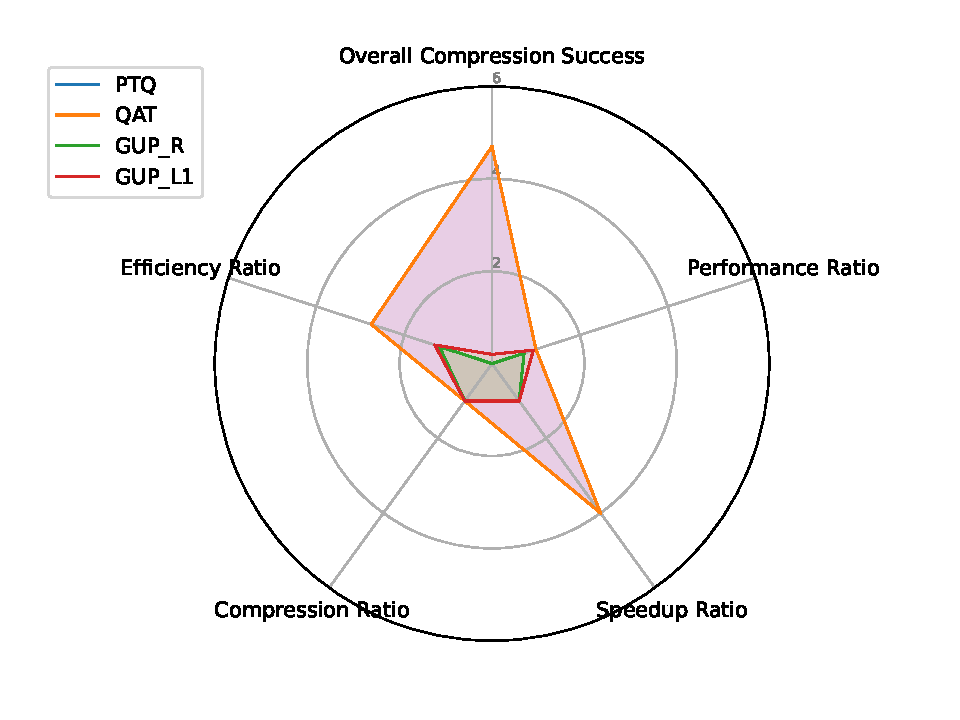
\includegraphics[width=1\textwidth]{other/figures/spider_pc_resnet18.pdf}
        \caption{}
    \end{subfigure}
    \begin{subfigure}{0.49\textwidth}
        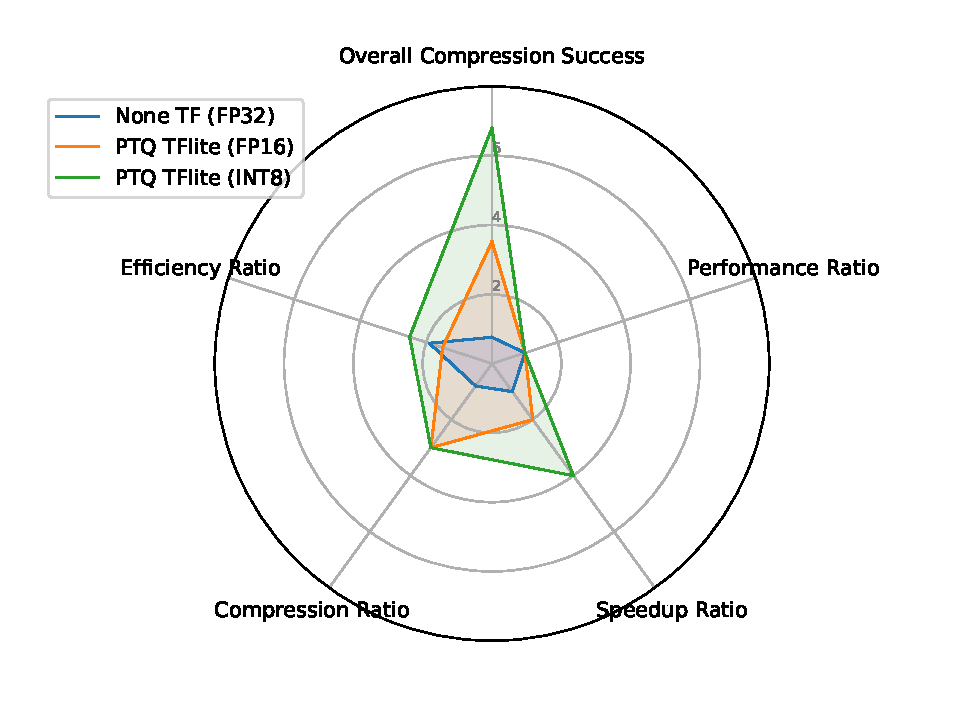
\includegraphics[width=1\textwidth]{other/figures/spider_raspebrrypi_yolo.pdf}
        \caption{}
    \end{subfigure}
   
    \caption{Radar plots summarising improvement ratios for (a) case study 1 and (b) for case study 2. The following summarises the metrics used in calculating the improvement ratios: Performance Ratio (Top1 for object classification and mAP for object detection),  Speedup Ratio (CHATS), Compression Ratio (CPU utilisation), Efficiency Ratio (Energy).}
    \label{fig:Radar-spider}
\end{figure*}




\section{Conclusions and Future Works} \label{sec:Conclusions}
In this paper we have provided a review of evaluation metrics for neural networks compression, with the aim of standardising evaluation of neural network compression. 
%
The metrics are grouped into five categories: Accuracy, Speed, Size, Energy, and Combined Measures.
%
The metrics reviewed were implemented and included in a compression bench library and named NetZIP, available publicly.
%
We identified lacking metrics that are needed to achieve more effective comparisons between compression techniques. Two novel evaluation metrics were contributed to cover the gap identified: 1) Compression and Hardware Agnostic Theoretical Speed (CHATS) and 2) Overall Compression Success (OCS). 
%
Furthermore, we used NetZIP to demonstrate the usage of reviewed and contributed metrics in two different case studies focusing on object classification, and object detection using two hardware platforms, a regular PC and a Raspberry pi 4.

Throughout the development of this work we used Quantisation and Pruning as the compression strategies on a limited number of neural network architectures. A future work is to expand NetZIP to include other compression strategies (e.g. Knowledge Distillation, Tensor Decomposition) and more neural network architectures.
%
Expanding to natural language processing (NLP) applications is another area for expanding in future works.
% Additionaly, we mainly focussed on vission aplications in our work and scope for expanding to other applications e.g. Natural langale preocessing (NLP) 

Carrying this work out we have identified other interesting areas of research that seem to not have attracted a lot researchers interests. 
%
Currently, pruning techniques only zero parameters but pruned parameters are not removed from the model architecture automatically, as removal of parameters from an architecture can result in errors.
%
There is need for developing model agnostic techniques for removal of pruned parameters.
%
Additionally, there is still scope for development of new metrics focused on  verification transferability pre- and post-compression to quantify functional equivalence.
%
Furthermore, there is need for doing more feasibility studies for utilisation of compressed models on edge devices. 




\section{Acknowledgements}
The work has been funded by the Thales Bristol Partnership in Hybrid Autonomous Systems Engineering (T-B PHASE).
%
This paper is based upon work from the COST Action no. CA19135 ``Connecting Education and Research Communities for an Innovative Resource Aware Society (CERCIRAS)", supported by the European Commission through the European Cooperation in Science and Technology (COST) Association.
% \balance

% ***************************************************
%  Bib
% ***************************************************
\printbibliography

% ***************************************************
%  Appendix
% ***************************************************

\end{document}
% \grid
